\documentclass{beamer}
\mode<presentation>
\usepackage{amsmath}
\usepackage{amssymb}
%\usepackage{advdate}
\usepackage{adjustbox}
\usepackage{subcaption}
\usepackage{enumerate}
\usepackage{multicol}
\usepackage{mathtools}
\usepackage{gvv}
\usepackage{listings}
\usepackage{url}
\def\UrlBreaks{\do\/\do-}
\usetheme{metropolis}
\setbeamertemplate{footline}
{
  \leavevmode%
  \hbox{%
  \begin{beamercolorbox}[wd=\paperwidth,ht=2.25ex,dp=1ex,right]{author in head/foot}%
    \insertframenumber{} / \inserttotalframenumber\hspace*{2ex} 
  \end{beamercolorbox}}%
  \vskip0pt%
}
\setbeamertemplate{navigation symbols}{}

\providecommand{\nCr}[2]{\,^{#1}C_{#2}} % nCr
\providecommand{\nPr}[2]{\,^{#1}P_{#2}} % nPr
\providecommand{\mbf}{\mathbf}
\providecommand{\pr}[1]{\ensuremath{\Pr\left(#1\right)}}
\providecommand{\qfunc}[1]{\ensuremath{Q\left(#1\right)}}
\providecommand{\sbrak}[1]{\ensuremath{{}\left[#1\right]}}
\providecommand{\lsbrak}[1]{\ensuremath{{}\left[#1\right.}}
\providecommand{\rsbrak}[1]{\ensuremath{{}\left.#1\right]}}
\providecommand{\brak}[1]{\ensuremath{\left(#1\right)}}
\providecommand{\lbrak}[1]{\ensuremath{\left(#1\right.}}
\providecommand{\rbrak}[1]{\ensuremath{\left.#1\right)}}
\providecommand{\cbrak}[1]{\ensuremath{\left\{#1\right\}}}
\providecommand{\lcbrak}[1]{\ensuremath{\left\{#1\right.}}
\providecommand{\rcbrak}[1]{\ensuremath{\left.#1\right\}}}
\theoremstyle{remark}

\providecommand{\abs}[1]{\left\vert#1\right\vert}
\providecommand{\res}[1]{\Res\displaylimits_{#1}} 
\providecommand{\norm}[1]{\lVert#1\rVert}
\providecommand{\mtx}[1]{\mathbf{#1}}
\providecommand{\mean}[1]{E\left[ #1 \right]}
\providecommand{\fourier}{\overset{\mathcal{F}}{ \rightleftharpoons}}
%\providecommand{\hilbert}{\overset{\mathcal{H}}{ \rightleftharpoons}}
\providecommand{\system}{\overset{\mathcal{H}}{ \longleftrightarrow}}
	%\newcommand{\solution}[2]{\textbf{Solution:}{#1}}
%\newcommand{\solution}{\noindent \textbf{Solution: }}
\providecommand{\dec}[2]{\ensuremath{\overset{#1}{\underset{#2}{\gtrless}}}}

\let\vec\mathbf

\lstset{
%language=C,
frame=single, 
breaklines=true,
columns=fullflexible
}

\numberwithin{equation}{section}

\title{Probability}
\author{Aditya Tripathy\\ Dept. of Electrical Engg.,\\IIT Hyderabad.}

\date{\today} 
\begin{document}

\begin{frame}
\titlepage
\end{frame}

\section*{Outline}
\begin{frame}
\frametitle{Table Of Contents}
\tableofcontents
\end{frame}
\section{Problem}
\begin{frame}
\frametitle{Problem Statement}
A coin is tossed twice, what is the probability that atleast one tail occurs?
%A circle $C$ passes through 
%\begin{equation} 
%\vec{P}=\myvec{-2\\ 4} 
%\label{eq:circle_7_p}
%\end{equation} 
%and touches the $y$-axis at 
%\begin{equation} 
%\vec{Q}=\myvec{0\\ 2}. 
%\label{eq:circle_7_q}
%\end{equation}
%Which one of the  following equations can represent a diameter of this circle?
%\begin{enumerate}[label=(\roman*)]
%\begin{multicols}{2}
%\setlength\itemsep{1em}
%\item $\myvec{4 & 5}\vec{x} = 6 $
%\item $\myvec{2 & -3}\vec{x} +10 = 0 $
%\item $\myvec{3 & 4}\vec{x} = 3 $
%\item $\myvec{5 & 2}\vec{x} +4= 0 $
%\end{multicols}
%\end{enumerate}
\end{frame}

%\subsection{Literature}
\section{Defining the random variables}
\begin{frame}
  \frametitle{Formulate in terms of bernoulli}
Let Y be the random variable representing the number of tails. Y can be represented as the sum of two bernoulli random variables, $X_1, X_2$,
\begin{align}
  Y = X_1 + X_2
\end{align}
The Bernoulli R.V is defined as,
\begin{align}
	X_i = \begin{cases}
		0 & \text{Outcome is Heads}\\	
		1 & \text{Outcome is Tails}	
	\end{cases}
\end{align}
%\framesubtitle{Literature}
%Let $\vec{O}$ be the centre of $C$. Then the equation of the normal, OQ is
%\begin{align}
%%\vec{x}^T\vec{x}-2\vec{O}^T\vec{x} +F = 0
%\myvec{0 & 1}\brak{\vec{O}-\vec{Q}} &= 0
%\nonumber \\ 
%\implies \myvec{0 & 1}\vec{O} = 2
%\label{eq:circle_7_o1}
%\end{align}
%%
%Also, 
%%Substituting \eqref{eq:circle_7_p} in \eqref{eq:circle_7_c}, 
%\begin{align}
%\norm{\vec{O}-\vec{P}}^2&=\norm{\vec{O}-\vec{Q}}^2 
%\nonumber \\
%\implies 2\brak{\vec{P}-\vec{Q}}^T\vec{O} &= \norm{\vec{P}}^2-\norm{\vec{Q}}^2 
%\nonumber \\
%\text{or, } \myvec{1 & -1}\vec{O} &= -4
%\label{eq:circle_7_o2}
%\end{align}
%%
%\eqref{eq:circle_7_o1} and \eqref{eq:circle_7_o2} result in the matrix equation
%\begin{align}
%\myvec{1 & -1 \\ 0 & 1}\vec{O} = \myvec{-4\\2}
%\label{eq:circle_7_matrix}
%\end{align}
%yielding the augmented matrix
%\begin{align}
%\myvec{1 & -1 & -4\\ 0 & 1 & 2} \leftrightarrow \myvec{1 & 0 & -2\\ 0 & 1 & 2}\implies \vec{O} = \myvec{-2 \\2}
%\label{eq:circle_7_o}
%\end{align}
%%
\end{frame}
\begin{frame}
\frametitle{PMF of bernoulli}
The PMF of Bernoulli R.V is given by,
\begin{align}
  p_X\brak{n} = \begin{cases}
    p & n = 0\\
    1-p & n = 1
  \end{cases}
\end{align}
%\begin{enumerate}[label=(\roman*)]
%\item $\myvec{4 & 5}\vec{O} = 2 \ne 6 $. Incorrect.
%\vfill
%\item $\myvec{2 & -3}\vec{O} +10 = 0 $. Correct.
%\vfill
%\item $\myvec{3 & 4}\vec{O} = 2 \ne 3 $.  Incorrect.
%\vfill
%\item $\myvec{5 & 2}\vec{O} +4= -2 \ne 0 $. Incorrect
%\end{enumerate}

\end{frame}
\begin{frame}
\frametitle{Z-transform to compute binomial PMF}

Using properties of Z transform of PMF on eq. \brak{0.1},
\begin{align}
  M_Y\brak{z} &= M_{X_1}\brak{z}M_{X_2}\brak{z}\\
  M_{X_1}\brak{z} &= \sum_{k = -\infty}^{\infty} p_{X_1}\brak{k}z^{-k} = p + \brak{1-p}z^{-1}\\
  M_{X_2}\brak{z} &= \sum_{k = -\infty}^{\infty} p_{X_2}\brak{k}z^{-k} = p + \brak{1-p}z^{-1}\\
  M_Y\brak{z} &= \brak{p + \brak{1-p}z^{-1}}^2\\
              &= \sum_{k = -\infty}^{\infty} \comb{2}{k}p^{2-k}\brak{1-p}^{k}z^{-k}\\
  p_Y\brak{n} &= \comb{2}{n} p^{2-n}\brak{1-p}^n
\end{align}
\end{frame}
\begin{frame}
\frametitle{Final PMF of Binomial distribution}
Substituting $p = \frac{1}{2}$,
\begin{align}
  p_Y\brak{n} &= \comb{2}{n}\brak{\frac{1}{2}}^2
\end{align}
\end{frame}
\section{CDF of binomial distribution}
\begin{frame}
\frametitle{CDF as a sum of PMF}
Using eq. (0.9) the CDF (Cumulative Distribution Function) is given by:
\begin{multline}
  F_{X}\brak{n}= \sum_{k = -\infty}^n\comb{2}{k}\brak{\frac{1}{2}}^2 =\\ \begin{cases}
    0 & x < 0\\
    \comb{2}{0}\brak{\frac{1}{2}}^2 = \frac{1}{4} & 0 \le x < 1\\
    \comb{2}{1}\brak{\frac{1}{2}}^2 + \comb{2}{0}\brak{\frac{1}{2}}^2 = \frac{3}{4}& 1 \le x < 2\\
    \comb{2}{2}\brak{\frac{1}{2}}^2 + \comb{2}{1}\brak{\frac{1}{2}}^2 + \comb{2}{0}\brak{\frac{1}{2}}^2 = 1 & x >=2\\
  \end{cases}
\end{multline}
\end{frame}
\begin{frame}
\frametitle{Back to the problem}
\begin{align}
  \pr{X \ge 1} &= 1 - F_X\brak{1}\\
  &= 1 - \frac{1}{4} = \frac{3}{4}
\end{align}
\end{frame}

\section{Simulating random bits with known bias}
\begin{frame}
\frametitle{Random bits}
To run a simulation we need to generate random numbers with uniform probability, which is done
as shown below(Algorithm taken from OpenSSL's random\_uniform.c):
\begin{enumerate}
  \item \text{Generate 1byte(8 bits) of entropy using OpenSSL/rand.h.}
  \item Scale down this number in the range [0, 255] to [0, 1]by dividing by 255.
  \item Return 0 if the scaled down number is less than p and return 1 otherwise. 
\end{enumerate}
\end{frame}
\begin{frame}
\frametitle{PMF of random variable}
\begin{figure}[h!]
   \centering
   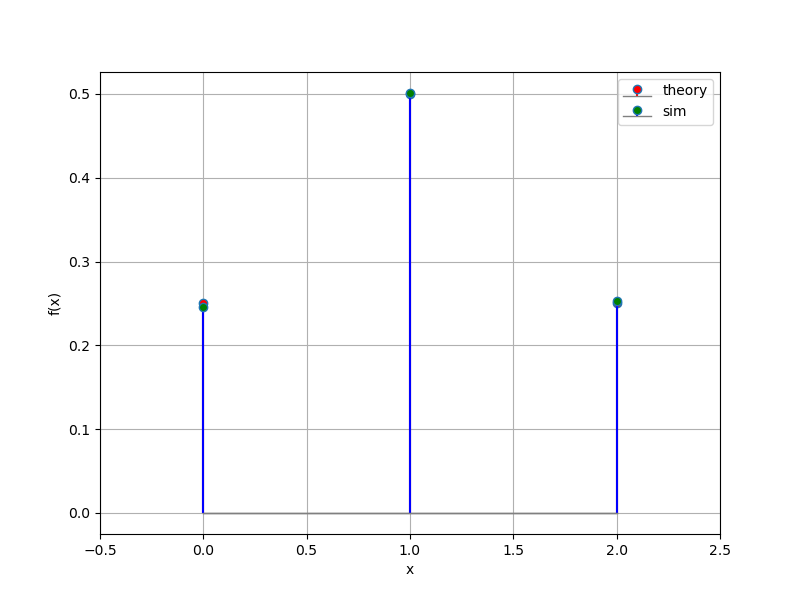
\includegraphics[width=0.7\columnwidth]{figs/fig1.png}
    \caption{Probability Mass Function}
\end{figure}

\end{frame}
\begin{frame}
  \frametitle{CDF of random variable}
\begin{figure}[h!]
   \centering
   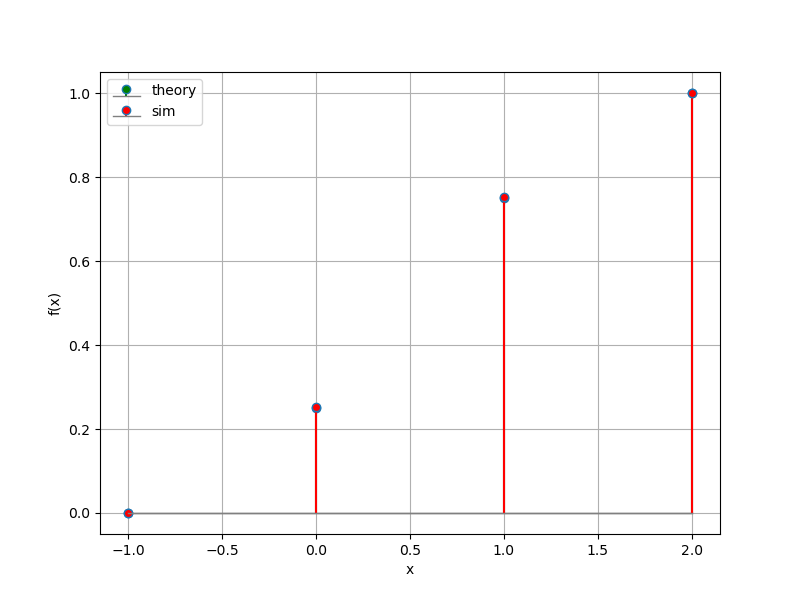
\includegraphics[width=0.7\columnwidth]{figs/fig2.png}
    \caption{Cumulative Distribution Function}
\end{figure}
\end{frame}
\begin{frame}
  \frametitle{Generating Binomial distribution for higher n}
\begin{figure}[h!]
   \centering
   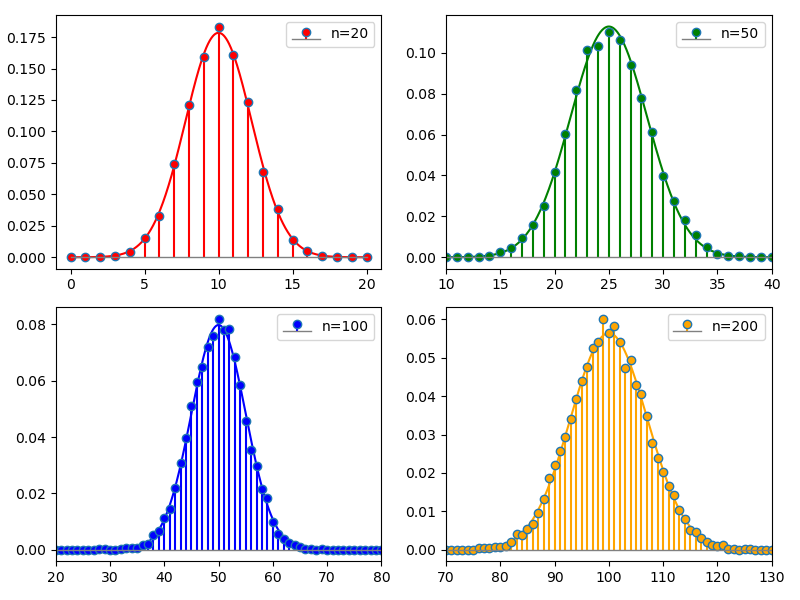
\includegraphics[width=0.7\columnwidth]{figs/binomial.png}
    \caption{Generating binomial distribution from bernoulli}
\end{figure}
\end{frame}
%\section{Plot}
\end{document}
